\documentclass[serif,final,bigger]{beamer}
\usepackage{enumerate}
\usepackage{graphicx}

\usetheme{Rochester}
\usecolortheme{beaver}
\linespread{1.6}  % Double spacing
\graphicspath{{../figures/}}

\title{Forecasting Lost Person Survival}
\author{Jonathan Lee}
\institute{TJHSST Computer Systems Lab}
\date{June 2, 2016}

\begin{document}
  \usebackgroundtemplate{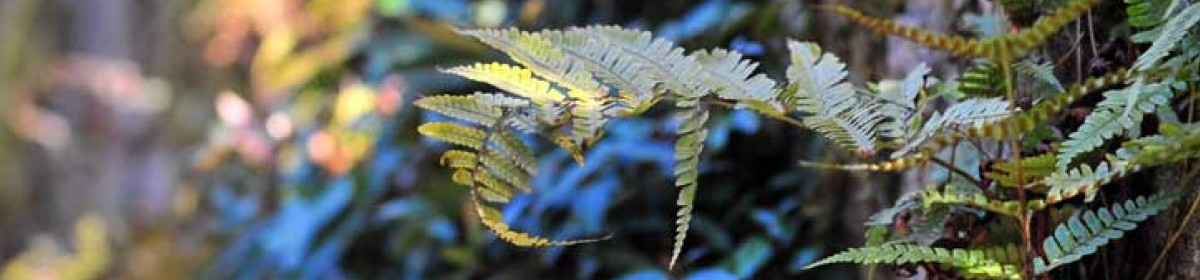
\includegraphics[width=\paperwidth]{ferns}}
  \begin{frame}
    \titlepage
  \end{frame}
  \usebackgroundtemplate{}

  \section{Introduction}

  \begin{frame}
    \frametitle{Purpose}
    \begin{itemize}
      \item Inform wilderness search-and-rescue (WiSAR) personnel when to terminate a search
      \item Augment lost person motion models
    \end{itemize}
  \end{frame}

  \begin{frame}
    \frametitle{Goals}
    \begin{itemize}
      \item Classify subjects as alive or dead-on-arrival (DOA)
      \item Generate probability-of-survival curves over time
    \end{itemize}
  \end{frame}

  \section{Methods}

  \begin{frame}
    \frametitle{Evaluation}
    \begin{itemize}
      \item Brier Score
      $$0 \leq \frac{1}{N} \sum_{i=1}^N (f_i - o_i)^2 \leq 1$$
    \end{itemize}
  \end{frame}

  \section{Results}

  \section{Conclusion}

  \begin{frame}
    \frametitle{Future Work}
  \end{frame}

  \section{Appendix}

  \begin{frame}
    \frametitle{References}
  \end{frame}
\end{document}
